\documentclass[tikz]{standalone}
\usepackage{pgfplots}
\pgfplotsset{compat=1.15}
\usepackage{mathrsfs}
\usetikzlibrary{arrows,calc}
\usepackage{tkz-euclide}

\pagestyle{empty}

\definecolor{AngleClr}{rgb}{0,0.39215686274509803,0}
\definecolor{ShapeClr}{rgb}{0.6,0.2,0}

\begin{document}

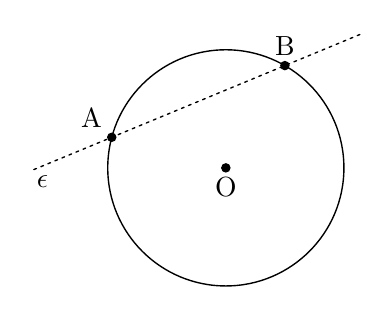
\begin{tikzpicture}[scale=.75]
\tkzSetUpLine[line width=1pt,color=black]
\tkzSetUpPoint[fill=black]

\tkzDefPoints{0/0/O}

\tkzDefPoint(165:2){A}
\tkzDefPoint(60:2){B}

\tkzDefPointOnLine[pos=-0.4](A,B)\tkzGetPoint{eps}


\tkzDrawSegments[line width=0.5pt,color=black,dashed,dash pattern=on 1pt off 1.75pt,add=.45 and .45](A,B)

\tkzDrawCircle[color=black,line width=0.5pt](O,A)


\tkzDrawPoints[size=3](O,A,B)
\tkzLabelPoint[above left](A){$\rm A$}
\tkzLabelPoint[above](B){$\rm B$}
\tkzLabelPoint[below](O){$\rm O$}
\tkzLabelPoint[below](eps){$\rm \epsilon$}

\end{tikzpicture}

\end{document}
